\documentclass[t,11pt]{beamer} % 8pt -- 14pt, 17pt and 20pt
\usetheme{bjtu}
\usecolortheme{bjtucolor}

% packages
\usepackage{graphicx}
\graphicspath{ {./images/} {./logo/}}
\usepackage{caption}
\usepackage{booktabs}
\usepackage{xeCJK}
\usepackage{fontspec}
\setCJKmainfont{HWzhongsong.ttf}
\setCJKmonofont{HWzhongsong.ttf}
\setromanfont{Times New Roman}
\setsansfont{Arial}

\usepackage[english]{babel}
\usepackage{xcolor}
\usepackage{amsmath}
\usepackage{textpos}
\usepackage{float}
\usepackage{hyperref}
% \hypersetup{
%     colorlinks=true,
%     linkcolor=blue,
%     filecolor=magenta,      
%     urlcolor=cyan,
% }


% show toc before each chapter
\AtBeginSection[]
{
  \begin{frame}
    \frametitle{Table of Contents}
    \setcounter{tocdepth}{2} % do not show subsection in toc
    \tableofcontents[currentsection]
    \addtocounter{framenumber}{-1}  % do not count in toc
  \end{frame}
}

% title,author,data etc.
\title{Title of the Presentation}
\subtitle{Subtitle}
\institute{\url{https://github.com/xuyangcao}}
\author{Xuyang Cao}
\date{2020.07.03}



% document body
\begin{document}
% title
\frame[plain]{\titlepage \addtocounter{framenumber}{-1}}        
% logo
\logo{
\includegraphics[width=1cm,height=1cm]{logo_bjtu}}

% table of contents
% comment this section if unnecessary
\begin{frame}{Table of Contents}           % table of contents frame 
    \setcounter{tocdepth}{2}               % do not show subsection
    \tableofcontents                       % table of contents
\end{frame}

% =====================
% generally, you do not need to change the document body any more
% please edit body.tex directly
\section{Section 1}
\begin{frame}[c]{Test Frame} % 参数c表示内容垂直居中,默认是顶部对齐[t]
    这是参考文献测试\cite{Cheplygina2018NotsosupervisedAS}
    
    这是一段中文测试
    
    公式:
    \[Dice = \frac{2 |A \cap B|}{|A| + |B|}\]
\end{frame}
 
\section{Section 2}
\begin{frame}[c]{Frame Title}
    \begin{columns}
    \column{0.5\textwidth}
    This is a text in first column.
    $$E=mc^2$$
    \begin{itemize}
    \item First item
    \item Second item
    \end{itemize}
     
    \column{0.5\textwidth}
    This text will be in the second column
    and on a second tought this is a nice looking
    layout in some cases.
    \end{columns}
\end{frame}


\begin{frame}{Frame Title}

\begin{columns}
\column{0.5\textwidth}
\begin{figure}
    \centering
    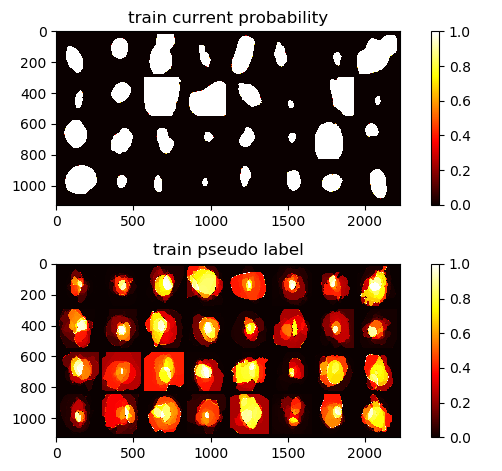
\includegraphics[width=1.\textwidth]{images/before.png}
    \caption*{Before}
\end{figure}

\column{0.5\textwidth}
\begin{figure}
    \centering
    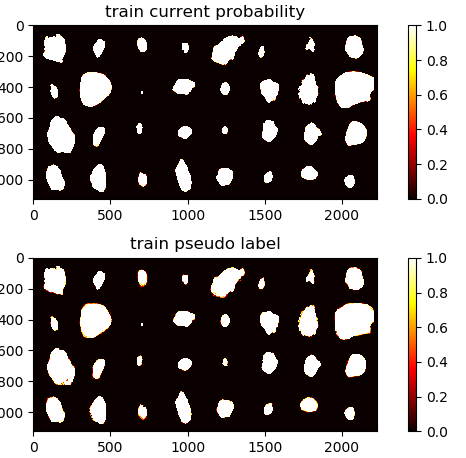
\includegraphics[width=1.\textwidth]{images/after.png}
    \caption*{After}
\end{figure}
\end{columns}
\end{frame}

\subsection{subsection 1} 
% =====================

% reference
% comment this section if unnecessary
\begin{frame}{Reference}
    \vspace{-0.5em}
    \nocite{*} % show all the reference
    \bibliographystyle{ieeetr}
    \tiny\bibliography{references}
\end{frame}

\end{document}